
\chapter{Request and response}

\section{Creating a project}

\lstset{language=Sh}
\begin{lstlisting}
  django-admin startproject mysite
\end{lstlisting}

This will create the files shown in Figure \ref{fig:startproject}:
\begin{figure}[!ht]
  \centering
  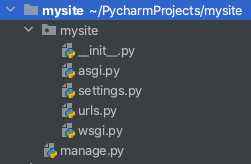
\includegraphics[width=\textwidth]{startproject.png}
  \label{fig:startproject}
  \caption{Start project}
\end{figure}


\section{The development server}
To start the project server to listen to all IPs on port 8000:
\begin{lstlisting}
  python manager.py runserver 0:8000
\end{lstlisting}

This will produce the following website Figure \ref{fig:runserver}:
\begin{figure}[!ht]
  \centering
  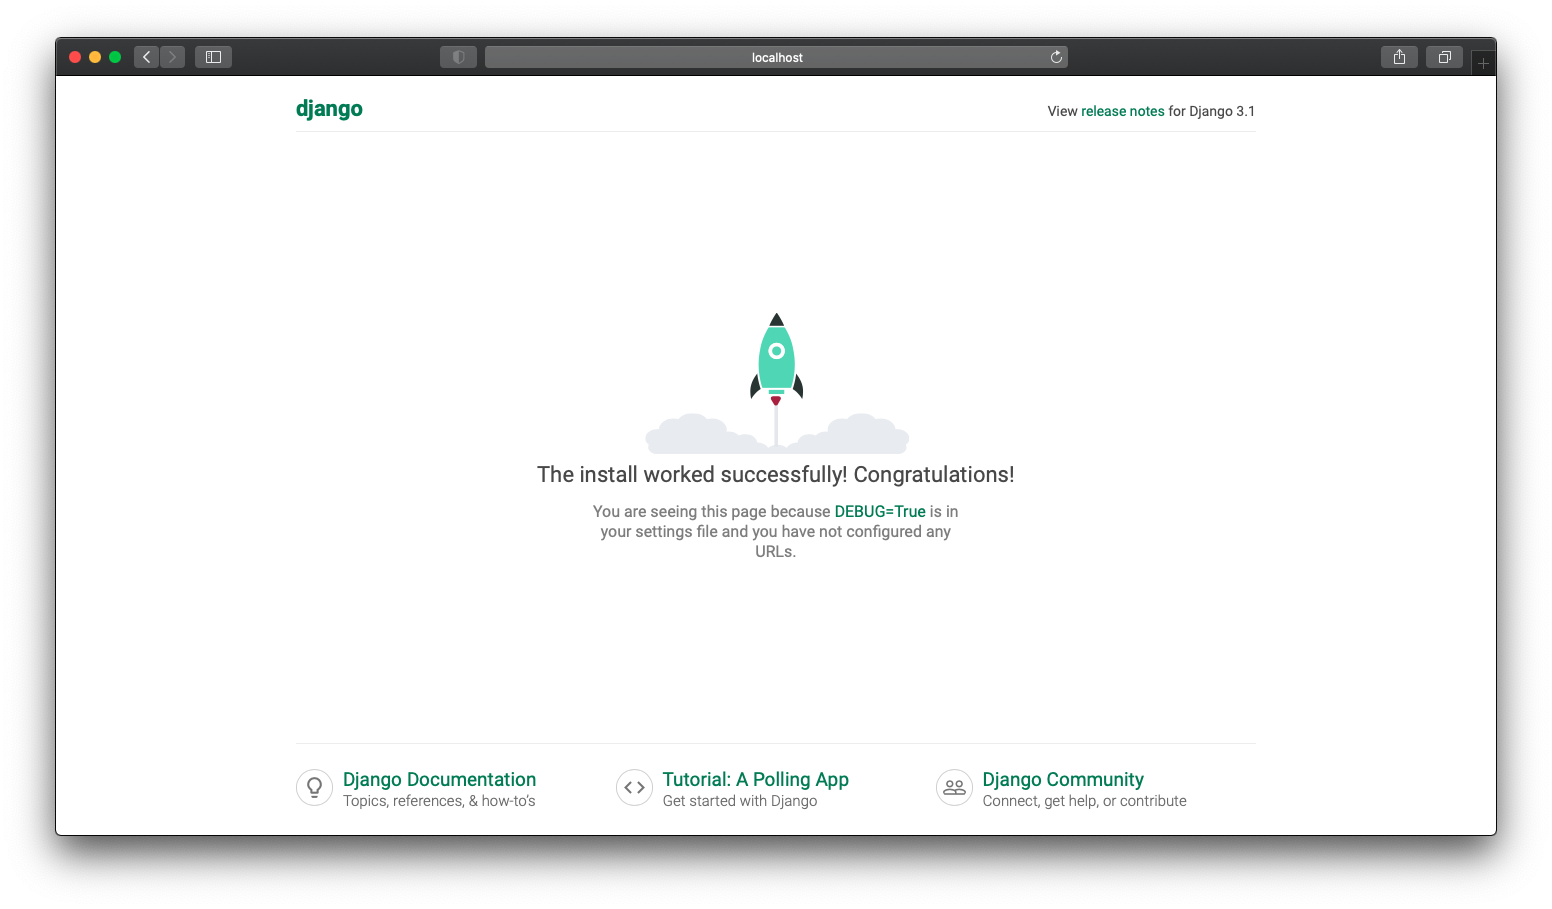
\includegraphics[width=0.9\textwidth]{runserver.png}
  \caption{Run server}
  \label{fig:runserver}
\end{figure}

\section{Creating an app}

Each application you write in Django consists of a Python package that follows a certain convention.
Django comes with a utility that automatically generates the basic directory structure of an app, so you can focus on writing code rather than creating directories.

\begin{lstlisting}
  python manage.py startapp pdfs
\end{lstlisting}


\section{Write your first view}

Open the file \keyword{polls/views.py} and put the following Python code in it:
\lstset{language=Python}
\begin{lstlisting}
from django.shortcuts import render
from django.http import HttpResponse


# Create your views here.
def index(request):
    return HttpResponse("Hello, world. You're at the polls index.")
\end{lstlisting}

  
To call the view, we need to map it to a URL - and for this we need a URL conf.


To create a URLconf in the polls directory, create a file called \keyword{polls/urls.py}.
In it include the following code:
\begin{lstlisting}
from django.urls import path

from . import views

urlpatterns = [
    path('', views.index, name='index'),
]
\end{lstlisting}


The next step is to point the root URLconf at the \keyword{polls.urls} module. In \keyword{mysite/urls.py}:
\begin{lstlisting}
from django.contrib import admin
from django.urls import path, include

urlpatterns = [
    path('polls/', include('polls.urls')),
    path('admin/', admin.site.urls),
]
\end{lstlisting}


Rerun the server and visit \url{http://localhost:8000/polls}.